\documentclass[manuscript,screen,review]{acmart}
\AtBeginDocument{%
  \providecommand\BibTeX{{%
    \normalfont B\kern-0.5em{\scshape i\kern-0.25em b}\kern-0.8em\TeX}}}
    
\usepackage{graphicx, subfigure}
\usepackage[ruled]{algorithm2e}

\newcommand{\assign}{\longleftarrow}
    
\begin{document}

\title{Using Polygonal Data Clusters to Investigate LIME}

\author{Jesse He}
\affiliation{%
  \institution{The Ohio State University}
  \city{Columbus}
  \state{Ohio}
  \country{USA}
}
\author{Subhasish Mazumdar}
\affiliation{%
  \institution{New Mexico Institute of Mining and Technology}
  \city{Sorocco}
  \state{New Mexico}
  \country{USA}
}

\begin{abstract}
    As machine learning models become more widely adopted, it is important to be able to create interpretable
    explanations for these models' predictions. LIME is a popular explanation framework which, despite successes
    in text and image data, still has some difficulties with tabular data. We present a method for generating
    synthetic tabular datasets drawn from classes that can be described geometrically using polygons, and use this 
    method to try to investigate LIME's behavior on a classifier given classification tasks of various difficulties.
\end{abstract}

\begin{CCSXML}
<ccs2012>
   <concept>
       <concept_id>10011007.10011006.10011072</concept_id>
       <concept_desc>Software and its engineering~Software libraries and repositories</concept_desc>
       <concept_significance>500</concept_significance>
       </concept>
   <concept>
       <concept_id>10010147.10010257.10010258.10010259.10010263</concept_id>
       <concept_desc>Computing methodologies~Supervised learning by classification</concept_desc>
       <concept_significance>100</concept_significance>
       </concept>
 </ccs2012>
\end{CCSXML}

\ccsdesc[500]{Software and its engineering~Software libraries and repositories}
\ccsdesc[100]{Computing methodologies~Supervised learning by classification}

\keywords{synthetic data, polygonal boundaries, machine learning explanations}

\maketitle

\section{Introduction}

With the increasing success of machine learning in analyzing data and the rising potential for its
applications in diverse areas, the necessity for understandable explanations of machine learning predictions
has become readily apparent. A key tool in evaluating such explanations, and in machine learning more generally,
is the ability to generate synthetic data sets to use as easily visualizable examples of real machine learning problems.
One class of problems with $n$-dimensional data involves identifying classes whose boundaries can be described
geometrically using polygons, especially when the polygons are non-convex. Below, we will use the term ``polygonal cluster'' 
to refer to such a class of data points which is definable with a polygonal boundary, and the term ``polygonal clustering'' to refer to the task of classifying such data. We will also allow a polygonal cluster to have a certain fraction of outliers which lie outside the polygonal boundary.
This presents an interesting class of classification problem that currently lacks a robust synthetic data tool.

There are a number of efforts in the realm of explainable AI, particularly regarding ``opaque'' or ``black-box''
models \cite{xai-pp}. One popular approach is the use of Local Interpretable Model-agnostic Explanation (LIME)
\cite{lime}, which attempts to identify the contribution of individual features towards a classifier's prediction
by observing the behavior of the classifier around perturbations of the original data point. An intuitive
illustration from Ribeiro, Singh, and Guestrin \cite{lime} is given in Figure \ref{fig:lime}.
\begin{figure}[ht]
    \centering
    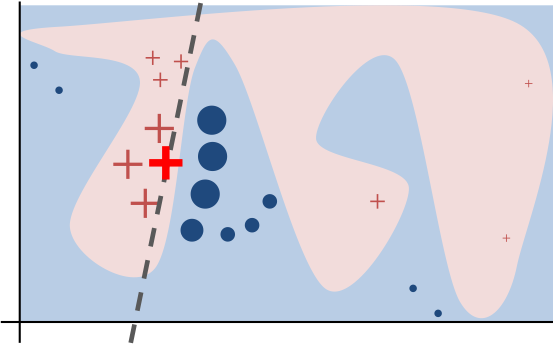
\includegraphics[width=.5\textwidth]{images/lime.png}
    \caption{
        Illustration to build intuition for LIME from Ribeiro, Singh, and Guestrin\cite{lime}.
        The lack-box model's prediction for the red cross is based on a complex decision boundary,
        illustrated by the blue/pink background. LIME samples nearby instances, gets the model's
        prediction, and attempts to create an explanation that is locally faithful.
    }
    \label{fig:lime}
\end{figure}

Although LIME has seen adoption in image and text analysis, LIME's application to tabular data
has certain limitations. Different methods of perturbing or identifying a local neighborhood for a data point
can create different explanations for the same classifier on the same dataset \cite{expma}, and Slack et al. 
\cite{fooling} have described a method for ``tricking'' LIME with an adversarial biased classifier whose biases
are undetected by LIME, which they argue is a weakness of similar post-hoc explainers. Because of the prevalence of
tabular data in machine learning applications, it is important to investigate LIME's ability to explain tabular
classification models.

One technique of interest is the use of a polygonal model, which attempts to create a suitable
polygon to represent the shape of a data cluster, often employed with spatial data \cite{polygon-mining}. Of particular 
interest are clusters bound by polygons which are non-convex, since convex hulls can create large empty areas that do 
not tightly fit the structure of a cluster. Although sample datasets exist that can be used for such problems, there is no 
robust way to randomly generate and customize new datasets with polygonal clusters. In this paper, we describe a software tool which uses a simple but effective method of generating such classification problems, and we demonstrate its utility in investigating the behavior of LIME on a black box classifier.

\section{Generating Clusters with Polygonal Boundaries}

In this section we describe briefly the method for generating polygonal clustering problems. More detailed pseudocode
can be found in Appendix \ref{algs}.

The first task in generating a polygonal clustering problem is to be able to generate polygons in the plane.
We can specify an $n$-gon $p$ as an ordered list $p = (v_1, v_2, \dots, v_n)$ of its vertices. In order to
generate these randomly we use a star-like approach: given a specified or randomly generated ``center'' we draw
a radius $r$ uniformly at random from some range $[r_m, r_M)$, where $0 \leq r_m < r_M$,
and an angle $\theta$ uniformly at random from $[0, 2\pi)$, giving us the polar coordinates for each vertex.
We then connect these vertices counter-clockwise to produce the polygon.

If we want to ensure that the polygon contains the central point about which it is generated, we
ensure that no consecutive angles $\theta_1$, $\theta_2$ have a difference of more than $\pi$ radians counter-clockwise.
For $n > 3$ we it suffices to generate the angle $\theta$ of the $k$-th vertex inside the interval
$[2(k-1)\pi / n, 2k\pi / n)$ for $n > 3$. For triangles, however, this may fail, so instead we generate the vertices
$(r_1, \theta_1)$, $(r_2, \theta_2)$, $(r_3, \theta_3)$, with $\theta_1$ selected uniformly at random from $[0, 2\pi)$ as before, then taking $\theta_2$ from $[\theta_1, \theta_1 + \pi)$, and $\theta_2$ from $[\theta_1 + \pi, \theta_2 + \pi)$.

Then given a polygon $p$, we wish to generate points that lie inside $p$. The simplest way to do this is by rejection
sampling: simply generate trial points and discard any that lie outside of $p$. Using this approach, we can draw
samples not just uniformly distributed from the polygon but also from a multivariate normal distribution centered
inside $p$, as well as allowing some number of points which lie outside of $p$. Of course, $p$ need not be generated randomly by the above process; the user may specify a polygon by enumerating its vertices.

Combining these techniques, we can easily generate random point sets with polygonal cluster boundaries. Our software uses Matplotlib's \texttt{path} library \cite{matplotlib} to represent polygonal paths and test if a polygon contains a given point. This also allows for easy visualization in plots made using Matplotlib and for integration with other Python libraries, including efficient vectorized operations with NumPy \cite{numpy}.
Examples are shown in Figures \ref{fig:make-poly} and \ref{fig:make-poly-diff}.
\begin{figure}[ht]
    \centering
    \parbox{.45\textwidth}{
        \begin{subfigure}
            \centering
            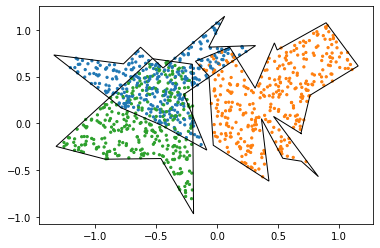
\includegraphics[width=.4\textwidth]{images/polygon_points.png}
            \caption{Three uniform balanced polygonal clusters.}
            \label{fig:make-poly}
        \end{subfigure}
    }
    \parbox{.45\textwidth}{
        \begin{subfigure}
            \centering
            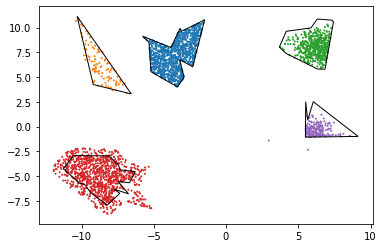
\includegraphics[width=.4\textwidth]{images/poly_diff.png}
            \caption{Customized clusters.}
            \label{fig:make-poly-diff}
        \end{subfigure}
    }
\end{figure}

\subsection{Controlling Overlap}

One additional task in generating new classification problems is to customize the difficulty of the problem.
The primary way we achieve this is by moving polygonal clusters closer or farther away from each other, and in
particular manipulating the \textit{overlap} between clusters. Given a set $X \subseteq \mathbb{R}^2$ of points
and regions $P_1$, $P_2$ bounded by polygons $p_1$ and $p_2$, respectively, we define the overlap between these
clusters by
\[
    \mathrm{overlap}(X, p_1, p_2) = \frac{|X \cap P_1 \cap P_2|}{|X|}.
\]
For problems with more than two polygons, we extend this definition by counting the number of points of $X$ that lie
in the intersection of any two polygons:
\[
    \mathrm{overlap}(X, p_1, \dots, p_k)
    = \frac{\left|X \cap \left(\bigcup_{1 \leq i < j \leq k} (P_i \cap P_j) \right) \right|}{|X|}.
\]
Then shifting clusters gives us control over the overlap of a classification problem, as seen in Figure \ref{fig:overlap_ex}.
By manipulating the overlap of our polygonal point sets, we can effectively scale the difficulty of the classification
problem: When there is no overlap, a simple linear model may suffice to accurately classify new test points. Introducing
overlap between clusters can give us insight into how classifiers create their decision boundaries in the presence of
ambiguous data.

\begin{figure}
    \centering
    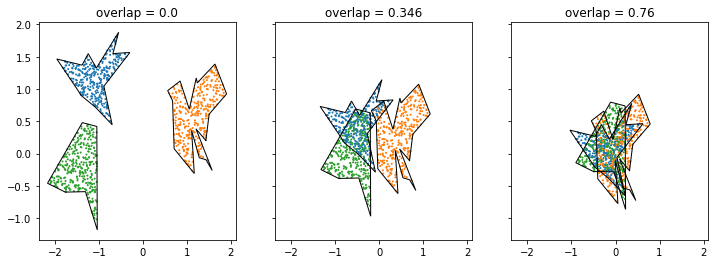
\includegraphics[width=.8\textwidth]{images/overlap.png}
    \caption{Dataset from Fig. \ref{fig:make-poly} with clusters shifted to create different overlaps.
    From left to right: dataset with no overlap, original dataset, dataset with high overlap}
    \label{fig:overlap_ex}
\end{figure}

\subsection{Polytopes in Higher Dimensions}

Real datasets frequently feature several features, of which some may be uninformative. In order to replicate
this we can sample points from polytopes of dimension $>2$, shown in Figure \ref{fig:3d_ex}. Currently in the software
these polytopes are specified by their orthogonal projections onto each standard coordinate plane, although this creates certain practical difficulties in implementation that are discussed further in Appendix \ref{nd-limits}. We can also generate new
redundant features by taking random linear combinations of existing features, and Gaussian noise can be added to
increase the difficulty of identifying redundant features, illustrated in Figure \ref{fig:extra-feature}.
\begin{figure}[ht]
    \centering
    \begin{subfigure}
        \centering
        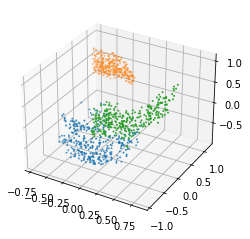
\includegraphics[width=.3\textwidth]{images/poly_3d.png}
        \label{poly-3d}
    \end{subfigure}
    
    \begin{subfigure}
        \centering
        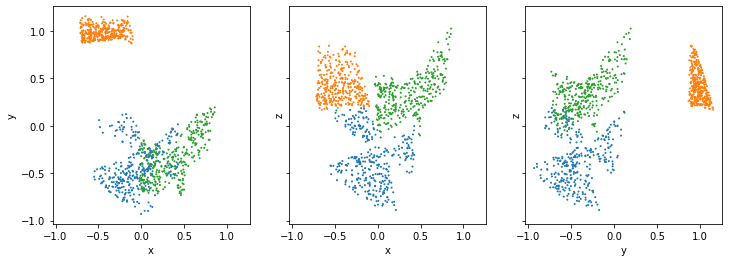
\includegraphics[width=.8\textwidth]{images/poly_3d_projs.png}
        \label{poly-3d-projs}
    \end{subfigure}
    \caption{A random clustering problem with polyhedral boundaries and its projections onto the
    $xy$, $xz$, and $yz$ planes.}
    \label{fig:3d_ex}
\end{figure}

\begin{figure}[ht]
    \centering
    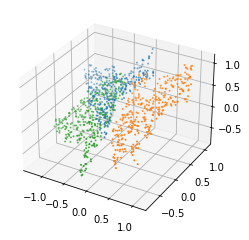
\includegraphics[width=.3\textwidth]{images/extra-feature.png}
    \caption{The dataset from Fig. \ref{fig:make-poly} with an artificial redundant feature.}
    \label{fig:extra-feature}
\end{figure}

\section{Explaining Classifier Behavior on Polygonal Clusters}

We first demonstrate the use of polygonal boundaries to specify challenging classification problems by creating a polygon
$p = ((.5, 0), (.7, 1), (.5,.2), (.3, 1), (.5, 0))$ and training a multilayer perceptron (MLP) classifier to classify points as inside or outside it.
We then select predictions in challenging areas and ask LIME to explain these predictions.
\begin{figure}
    \centering
    \begin{subfigure}
        \centering
        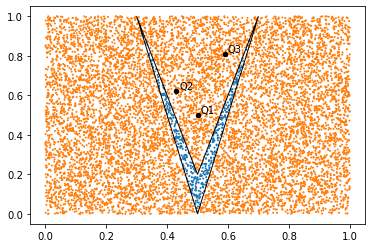
\includegraphics[width=.4\textwidth]{images/lime-corner-plot.png}
        \label{lime-corner-plot}
    \end{subfigure}
    \begin{subfigure}
        \centering
        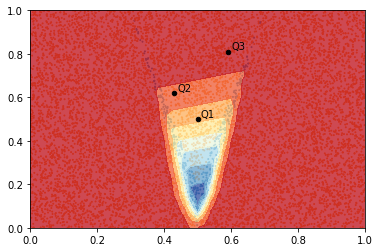
\includegraphics[width=.4\textwidth]{images/lime-corner-prob.png}
        \label{lime-corner-probs}
    \end{subfigure}
    \begin{subfigure}
        \centering
        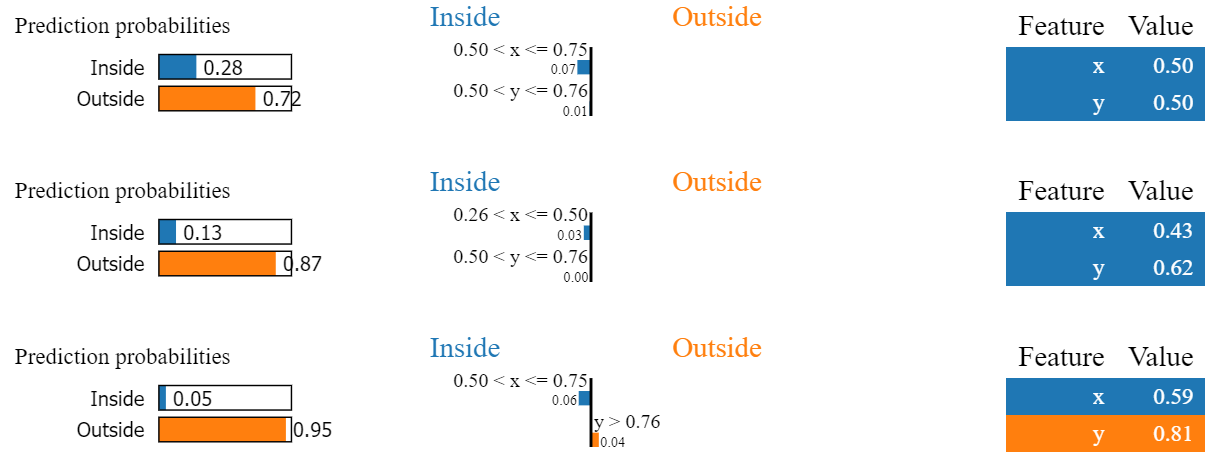
\includegraphics[width=.8\textwidth]{images/lime-corner-exps.png}
        \label{lime-corner-exps}
    \end{subfigure}
    \caption{
        A classification problem featuring a ``V''-like polygon with sample points $Q_1 = (0.5, 0.5), Q_2 = (.43, .62), Q_3 = (.59, .81)$ (top left), the classifier's decision function (top right), and LIME's explanations at $Q_1, Q_2$ , and $Q_3$ (bottom).
    }
    \label{fig:corner}
\end{figure}

As we can see in Figure \ref{fig:corner}, the inner triangle which is in the convex hull of $p$ but not within its boundaries is challenging for LIME to explain. Because LIME looks at individual features, its attempted explanations for the specified points contradicts the classifier's prediction: the classifier correctly identifies that each point lies outside $p$, but LIME's explanations suggest that each point \emph{should} be classified as inside the polygon based on their $x$ values.

Now, using our method of generating clusters we can demonstrate LIME's ability to identify the relevant feature in an easy clustering problem.
We create two polyhedral clusters whose $xy$ projections are nearly indistinguishable (an overlap of 0.633) but
which are separated by a plane through $z=0$. As Figure \ref{fig:3d_easy} shows, LIME can successfully identify
that the classifier only needs to use the $z$ coordinate to make its prediction.

\begin{figure}[ht]
    \centering
    \begin{subfigure}
        \centering
        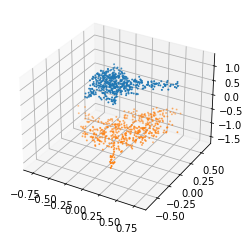
\includegraphics[width=.3\textwidth]{images/lime-3d-plot.png}
        \label{easy-3d}
    \end{subfigure}
    
    \begin{subfigure}
        \centering
        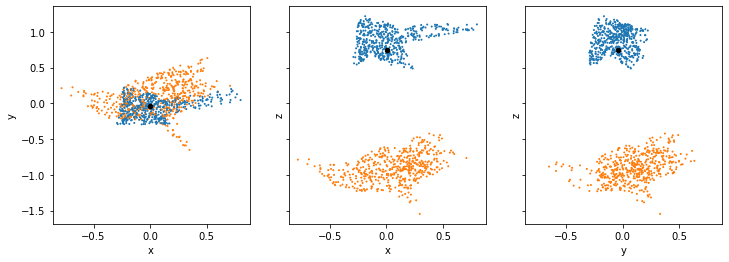
\includegraphics[width=.8\textwidth]{images/lime-3d-projs.png}
        \label{easy-3d-projs}
    \end{subfigure}
    
    \begin{subfigure}
        \centering
        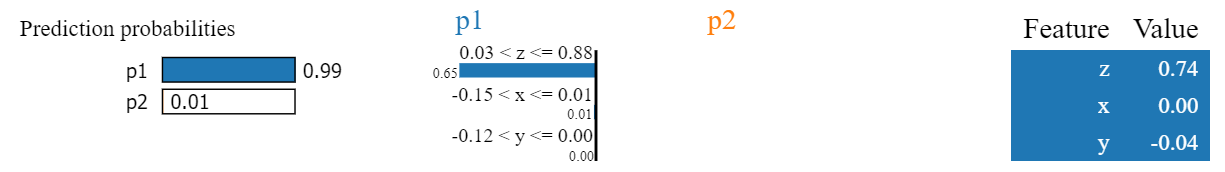
\includegraphics[width=.8\textwidth]{images/lime-3d-expl.png}
        \label{lime-easy}
    \end{subfigure}
    
    \caption{An easy 3d classification problem featuring two clusters that are linearly separable with a plot
    (top) and its $xy$, $xz$, and $yz$ projections (middle), along with LIME's explanation (bottom).}
    \label{fig:3d_easy}
\end{figure}

To investigate the efficacy of LIME in evaluating tabular data in 2 dimensions with the overlap we have defined, we
create a binary classification problem with two polygonal clusters $p1$ and $p2$ whose overlap is between $0.1$ and
$0.2$, and we train an MLP on a subset of the data. We then probe the classifier's 
prediction of a particular point using LIME and compare it to the classifier's actual decision function in Figure
\ref{fig:2d-nn}.

\begin{figure}
    \centering
    \begin{subfigure}
        \centering
        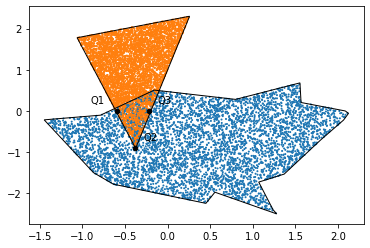
\includegraphics[width=.4\textwidth]{images/nn-lime-ex.png}
        \label{nn-lime}
    \end{subfigure}
    \begin{subfigure}
        \centering
        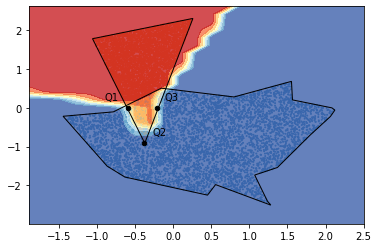
\includegraphics[width=.4\textwidth]{images/nn-prob-ex.png}
        \label{nn-prob}
    \end{subfigure}
    \begin{subfigure}
        \centering
        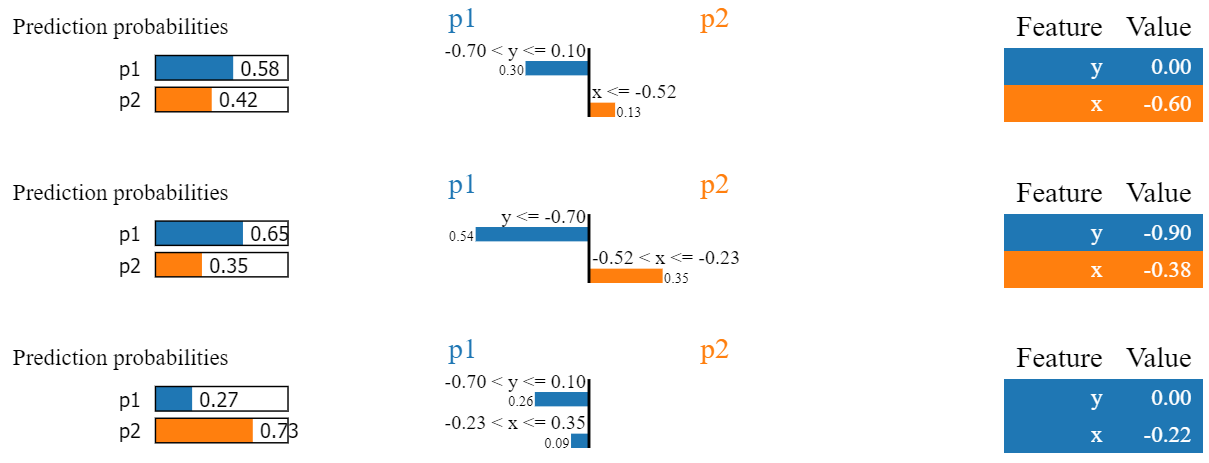
\includegraphics[width=.8\textwidth]{images/lime-exp.png}
        \label{lime-exp-2d}
    \end{subfigure}
    \caption{
        A binary polygonal classification problem. A plot of the dataset and polygons (top left) next to the classifier's
        decision boundary (top right). In both plots the points $Q_1 = (-0.6, 0)$, $Q_2 = (-0.38, -0.9)$,
        and $Q_3 = (-0.22, 0)$ are each marked by a red ``X.'' Below are LIME's explanations for the classifier's 
        predictions at these points.
    }
    \label{fig:2d-nn}
\end{figure}

All three points were chosen to be difficult for the classifier. Each lies within the boundaries of both $p1$ and $p2$
but is very close to the boundary of $p2$, and this difficulty is reflected when examining the classifier's decision
function. LIME's explanations at $Q_1$ and $Q_2$ reflect the classifier's uncertainty at those points, but its behavior
at $Q_3$ is unintuitive: the MLP classifies $Q_3$ in $p2$ with a probability of $0.73$, but LIME's explanation for
this prediction asserts that the $x$ and $y$ values are both in ranges correlated with $p1$. This explanation contradicts
the actual prediction of the classifier at $Q_3$, appearing to violate LIME's local faithfulness.


\section{Conclusion and Future Work}

This method of generating and manipulating polygonal tabular data is effective at generating simple example
datasets for clustering problems. The generated datasets are easily visualized and can be customized to fit different 
geometric and statistical structures. Using 
    polygons to specify the geometric structure allows for customization of
    cluster shape, and using overlap allows for customization of the difficulty
    of a generated classification problem.

In particular, our simple definition and manipulation of
overlap for polygonal clustering problems allows us to demonstrate surprising behavior with LIME. Although overlap
is currently only defined for polygonal clusters in two dimensions, the definition generalizes easily to other 
polytopes and a more refined computational approach may allow us to further investigate the behavior of LIME.

Future work could continue to develop this method of generating and manipulating tabular data with more features,
adding more robust support for higher-dimensional polytopes. In addition, these methods could be used to investigate
the behavior of other post-hoc black-box explainers like SHAP \cite{xai-pp}, as well as other classification methods
including polygonal modelling \cite{polygon-mining} or dimensionality reduction.

\begin{acks}
This work is supported by the National Science Foundation under grant 
no. CNS-1757945.
\end{acks}

\bibliographystyle{ACM-Reference-Format}
\bibliography{references}

\appendix

\section{Limitations in Higher Dimensions} \label{nd-limits}

The current approach to specifying a polytope in dimensions $> 2$ is based on its orthogonal projections: for example,
we specify a polyhedron by taking a polygon $p$ in the $xy$-plane and considering this in the $xz$- and $yz$-planes,
then taking the intersection of the cylinders created by extending these projections. In other words, a point $(x, y, z)$
is in the polytope if $p$ encloses $(x, y)$, $(x, z)$, and $(y, z)$ in two dimensions. This requires the polygon
be roughly centered on the line $y = x$, since otherwise there may be no points which satisfy this condition for a
given polygon, and even then generating points may be impossible. This also means that extending the overlap features
to higher dimensions requires either checking each $\binom{n}{2}$ projections of an $n$-dimensional polytope,
or would require a retooling of how polytopes are specified.

\section{Methods and Algorithms} \label{algs}

The data generation methods described in this paper have been implemented at \url{github.com/he-jesse/polydata}.
Interface design was based in part on the datasets module of the sci-kit learn project \cite{sklearn_api}
and the implementation uses a number of well-known Python libraries \cite{numpy, matplotlib, scikit-learn}.
This appendix contains pseudocode for simple versions of the two-dimensional algorithms. Note that the current
implementation supports additional features not described here.

\begin{algorithm}[ht]
\SetAlgoLined
\DontPrintSemicolon
\KwData{A number $n$ of vertices, a center $(x_0, y_0)$, a range $(r_m, r_M)$ of distances from the center to a vertex}
\KwResult{A polygon $p = (v_1, v_2, \dots, v_n)$}
\Begin{
    $p \assign ()$\;
    \For{$i \in \{1, \dots, n\}$}{
        $(r_i, \theta_i) \assign ($random$(r_m, r_M)$, random$(0, 2\pi))$
    }
    $V \assign$ sort$(r_i, \theta_i)$ by $\theta$\;
    \For{$(r_i, \theta_i) \in V$}{
        p.append($(r_i\cos(\theta_i) + x_0, r_i\sin(\theta_i) + y_0)$)
    }
    \KwRet{$p$}
}
\caption{RandomPoly\label{rand-poly}}
\end{algorithm}

\begin{algorithm}[ht]
\SetAlgoLined
\DontPrintSemicolon
\KwData{A number $n$ of samples, a polygon $p$}
\KwResult{A set $X$ of points with $|X| = n$ and $p.contains(X)$}
\Begin{
    $X \assign \varnothing$\;
    \While{$|X| < n$}{
        $x \assign$ random point in the bounding box of $p$\;
        \If{$p.contains(x)$}{
            $X \assign X \cup \{x\}$
        }
    }
    \KwRet{X}
}
\caption{SamplePoly\label{sample-poly}}
\end{algorithm}

\begin{algorithm}[ht]
\SetAlgoLined
\DontPrintSemicolon
\KwData{numSamples $n$, numPolygons $m$ of polygons, range $(r_m, r_M)$ to pass to Alg. \ref{rand-poly},
    a bounding box $B$}
\KwResult{A set $X$ of points, a set $P$ of polygons, and a map $f : X \to P$ so that $f(x).contains(x)$ for $x \in X$}
\Begin{
    $X, P \assign \varnothing$\;
    \For{$i \in \{1, \dots, m\}$}{
        $p \assign$ MakePoly(random($B$))\;
        $X_p \assign$ SamplePoly($p$)\;
        $X \assign X \cup X_p$\;
        $P \assign P \cup \{p\}$\;
        \For{$x \in X_p$}{
            $f \assign f \cup \{(x,p)\}$
        }
    }
    \KwRet{$X, P, f$}
}
\caption{MakePoly\label{make-poly}}
\end{algorithm}

\begin{algorithm}[ht]
\SetAlgoLined
\DontPrintSemicolon
\KwData{A point set $X$, a polygon set $P$}
\KwResult{The proportion $c$ of overlap}
\Begin{
    $Y \assign \varnothing$\;
    \For{$\{p_1, p_2\} \in P^{(2)}$}{
        \For{$x \in X$}{
            \If{$p_1$.contains($x$) and $p_2$.contains($x)$}{
                $Y \assign Y \cup \{x\}$
            }
        }
    }
    \KwRet{$|Y| / |X|$}
}
\caption{ComputeOverlap\label{comp-overlap}}
\end{algorithm}

\begin{algorithm}[ht]
\SetAlgoLined
\DontPrintSemicolon
\KwData{A point set $X$, a polygon set $P$, a function $f : X \to P$, a range $(c_m, c_M)$ of overlap values}
\KwResult{A point set $X'$ and polygon set $P'$ such that $c_m < $ overlap $< c_M$}
\Begin{
    $X' \assign X$
    $P' \assign P$
    $s_m \assign -1$\;
    $s_M \assign 1$\;
    $s \assign (s_m + s_M)/2$\;
    \While{$c_m > $overlap($X', P'$) or overlap($X', P'$)$ > c_M$}{
        \If{overlap($X', P'$) $< c_m$}{
            $s_M \assign s$
        }
        \ElseIf{overlap($X', P'$) $> c_M$}{
            \If{$s_M - s_m < \varepsilon$ \tcc*[r]{$\varepsilon$ is some small threshold}}{
                $s_M \assign s_M + 1$
            }
            $s_m = s$
        }
        $s \assign (s_m + s_M)/2$\;
        \For{$x \in X'$}{
            $x \assign x + s \cdot f(x)$.centroid())
        }
        \For{$p \in P'$}{
            $p \assign p + s \cdot p$.centroid()
        }
    }
    \KwRet{X', P'}
}
\caption{MakeOverlap\label{make-overlap}}
\end{algorithm}

\end{document}
\endinput

\end{document}